\documentclass[tikz,border=8pt]{standalone}
% Shared look for every TikZ diagram. Load with \input{../../tools/tikz-style.tex}
\usepackage[T1]{fontenc}
\usepackage{lmodern}
\renewcommand{\sfdefault}{lmr}  % diagrams use the same serif as the text
\usetikzlibrary{arrows.meta, positioning, shapes.geometric, calc, fit, backgrounds}
\definecolor{cblue}{HTML}{4C78A8}
\definecolor{corange}{HTML}{F58518}
\definecolor{cgreen}{HTML}{54A24B}
\definecolor{cred}{HTML}{E45756}
\definecolor{cpurple}{HTML}{B279A2}
\definecolor{cgrey}{HTML}{6B6B6B}
\tikzset{
  every picture/.style={font=\sffamily, line width=1.2pt},
  box/.style={draw=#1, fill=#1!12, rounded corners=4pt, align=center, inner sep=7pt, minimum height=1.1cm},
  box/.default=cgrey,
  arrow/.style={-{Stealth[length=3mm]}, draw=cgrey, line width=1.4pt},
  title/.style={font=\sffamily\bfseries\Large},
  note/.style={font=\sffamily\small, text=cgrey, align=center},
}
\AtBeginDocument{\hyphenpenalty=10000 \exhyphenpenalty=10000}

\begin{document}
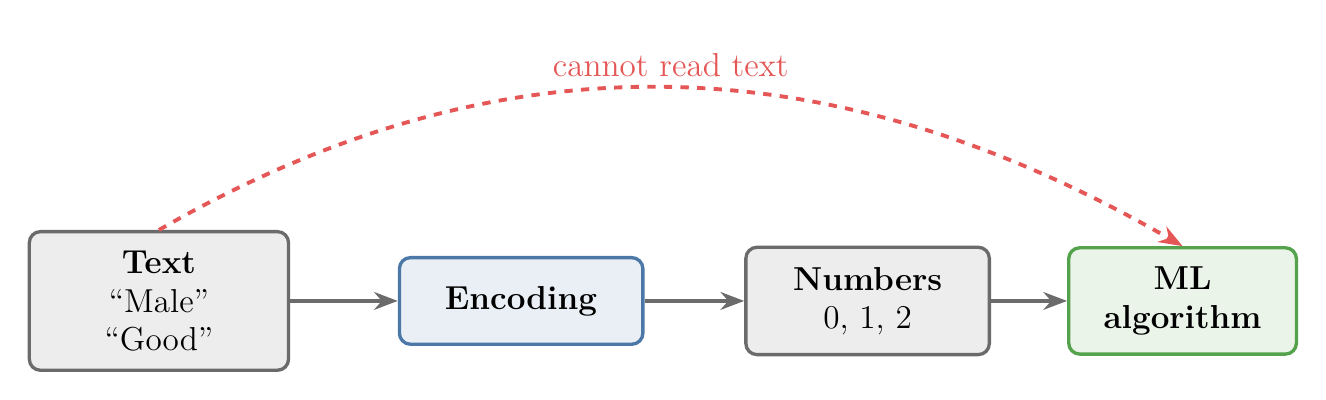
\begin{tikzpicture}[every node/.append style={font=\sffamily\large}]
\tikzset{note/.style={font=\sffamily\large, text=cgrey, align=center}}
  \node[box=cgrey, text width=2.8cm] (t) at (0,0) {\textbf{Text}\\``Male''\\``Good''};
  \node[box=cblue, text width=2.6cm] (e) at (4.6,0) {\textbf{Encoding}};
  \node[box=cgrey, text width=2.6cm] (n) at (9.0,0) {\textbf{Numbers}\\0, 1, 2};
  \node[box=cgreen, text width=2.4cm] (m) at (13.0,0) {\textbf{ML}\\\textbf{algorithm}};
  \draw[arrow] (t) -- (e); \draw[arrow] (e) -- (n); \draw[arrow] (n) -- (m);
  \draw[arrow, draw=cred, dashed] (t.north) to[out=30, in=150] node[above, text=cred] {cannot read text} (m.north);
\end{tikzpicture}
\end{document}
